% Digital Logic Report Template
% Created: 2020-01-10, John Miller

%==========================================================
%=========== Document Setup  ==============================

% Formatting defined by class file
\documentclass[11pt]{article}

% ---- Document formatting ----
\usepackage[margin=1in]{geometry}	% Narrower margins
\usepackage{booktabs}				% Nice formatting of tables
\usepackage{graphicx}				% Ability to include graphics

%\setlength\parindent{0pt}	% Do not indent first line of paragraphs 
\usepackage[parfill]{parskip}		% Line space b/w paragraphs
%	parfill option prevents last line of pgrph from being fully justified

% Parskip package adds too much space around titles, fix with this
\RequirePackage{titlesec}
\titlespacing\section{0pt}{8pt plus 4pt minus 2pt}{3pt plus 2pt minus 2pt}
\titlespacing\subsection{0pt}{4pt plus 4pt minus 2pt}{-2pt plus 2pt minus 2pt}
\titlespacing\subsubsection{0pt}{2pt plus 4pt minus 2pt}{-6pt plus 2pt minus 2pt}

% ---- Hyperlinks ----
\usepackage[colorlinks=true,urlcolor=blue]{hyperref}	% For URL's. Automatically links internal references.

% ---- Code listings ----
\usepackage{listings} 					% Nice code layout and inclusion
\usepackage[usenames,dvipsnames]{xcolor}	% Colors (needs to be defined before using colors)

% Define custom colors for listings
\definecolor{listinggray}{gray}{0.98}		% Listings background color
\definecolor{rulegray}{gray}{0.7}			% Listings rule/frame color

% Style for Verilog
\lstdefinestyle{Verilog}{
	language=Verilog,					% Verilog
	backgroundcolor=\color{listinggray},	% light gray background
	rulecolor=\color{blue}, 			% blue frame lines
	frame=tb,							% lines above & below
	linewidth=\columnwidth, 			% set line width
	basicstyle=\small\ttfamily,	% basic font style that is used for the code	
	breaklines=true, 					% allow breaking across columns/pages
	tabsize=3,							% set tab size
	commentstyle=\color{gray},	% comments in italic 
	stringstyle=\upshape,				% strings are printed in normal font
	showspaces=false,					% don't underscore spaces
}

% How to use: \Verilog[listing_options]{file}
\newcommand{\Verilog}[2][]{%
	\lstinputlisting[style=Verilog,#1]{#2}
}




%======================================================
%=========== Body  ====================================
\begin{document}

\title{ELC 2137 Lab 10: 7-segment Display with Time-Division Multiplexing}
\author{Alexander Noll}

\maketitle


\section*{Summary}

Building upon previous labs, we utilized registers and sequential logic to design timers. Using these timers, the calculator and 7-segment display driver were combined to create a 4 digit calculator with display. 


\section*{Q\&A}

1. The three main groups of the RTL definition of sequential logic include state memory, next-state, and output logic.
2. 
\begin{figure}[ht]\centering
	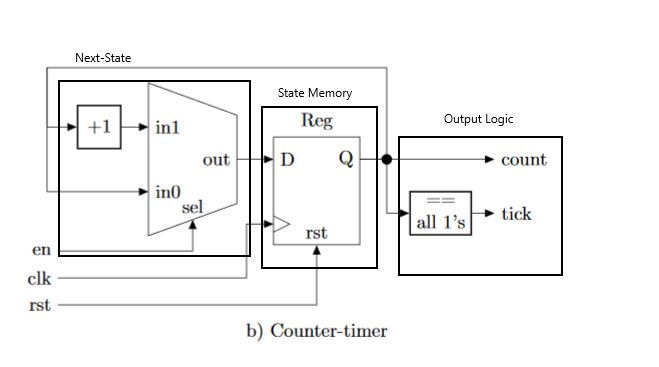
\includegraphics[width=1.0\textwidth,trim=0 0mm 0 0,clip]{Q2Pic}
	\caption{RTL Groups in a Counter Timer}
\end{figure}
3. Qnext={Qreg[N-2],1}.



\clearpage

\section*{Results}

\begin{table*}[ht]\centering
	\caption{\textit{register} expected results table}
	\label{ALU:tbl:register_ERT}\medskip
	\begin{tabular}{l|rrrrrrrrrrrrrrr}
		Time (ns): & 0-1 & 1-2 & 2-3 & 3-4 & 4-5 & 5-6 & 6-7 & 7-8 & 8-9 & 9-10 &10-11& 11-12 & 12-13 & 13-14 & 14-15\\
		\midrule
		clk     & 0 & 1 & 0 & 1 & 0 	& 1 & 0 & 1 & 0 & 1 	& 0 & 1 & 0 & 1 & 0\\
		en  	& 0 & 0 & 0 & 0 & 0 	& 0 & 1 & 1 & 1 & 1 	& 1 & 1 & 0 & 0 & 0\\
		rst 	& 0 & 0 & 0 & 1 & 1 	& 1 & 0 & 0 & 0 & 0 	& 0 & 0 & 0 & 0 & 0\\
		\midrule
		Q (dec) & X & X & X & 0 & 0 	& 0 & 0 & 1 & 1 & 2 	& 2 & 3 & 3 & 3 & 3\\
		tick & 0 & 0 & 0 & 0 & 0 	& 0 & 0 & 0 & 0 & 0 	& 0 & 0 & 0 & 0 & 0\\
		\bottomrule
	\end{tabular}
\end{table*}

\begin{figure}[ht]\centering
	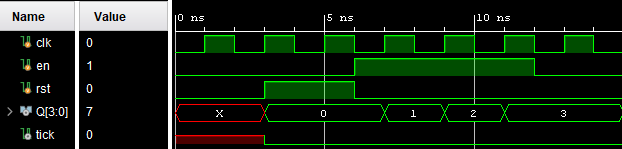
\includegraphics[width=1.0\textwidth,trim=0 0mm 0 0,clip]{CounterTest}
	\caption{Counter Test Waveform}
\end{figure}

\clearpage

\begin{table*}[ht]\centering
	\caption{\textit{alu} expected results table skeleton}
	\label{ALU:tbl:alu_ERT}\medskip
	\begin{tabular}{l|rrrrrrrrrrrrrrr}
		Clock Cycles:& 0-1 & 1-2 & 2-3 & 3-4 & 4-5 & 5-6 & 6-7 & 7-8 & 8-9 & 9-10 &10-11& 11-12 & 12-13 & 13-14 & 14-15\\
		\midrule
		Input  & 49 & 49 & 49 & 49 & 49 & 49 & 49 & 49 & 49 & 49 & 49 & 49 & 49 & 49 & 49\\
		Reset  & 0 & 0 & 0 & 0 & 0 	& 1 & 1 & 1 & 1 & 1 	& 0 & 0 & 0 & 0 & 0\\
		\midrule
		Seg	& 40 & 40 & 40 & 40 & 40 	& 30 & 30 & 30 & 30 & 30 	& 78 & 40 & 40 & 30 & 78\\
		an & X & X & X & X & X 	& e & e & e & e & e 	& d & b & 7 & e & d\\
		dp  & 1 & 1 & 1 & 1 & 1 	& 1 & 1 & 1 & 1 & 1 	& 1 & 1 & 1 & 1 & 1\\
		\bottomrule
	\end{tabular}
\end{table*}

\begin{figure}[ht]\centering
	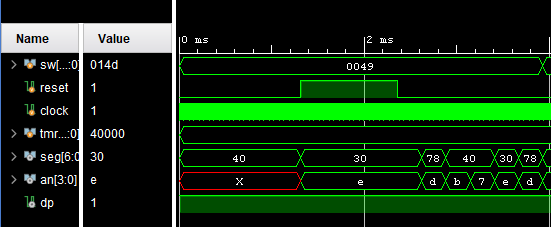
\includegraphics[width=1.0\textwidth,trim=0 0mm 0 0,clip]{SsegTDMTest}
	\caption{7-Segment Driver Test Waveform}
\end{figure}


	
\begin{figure}[ht]\centering
	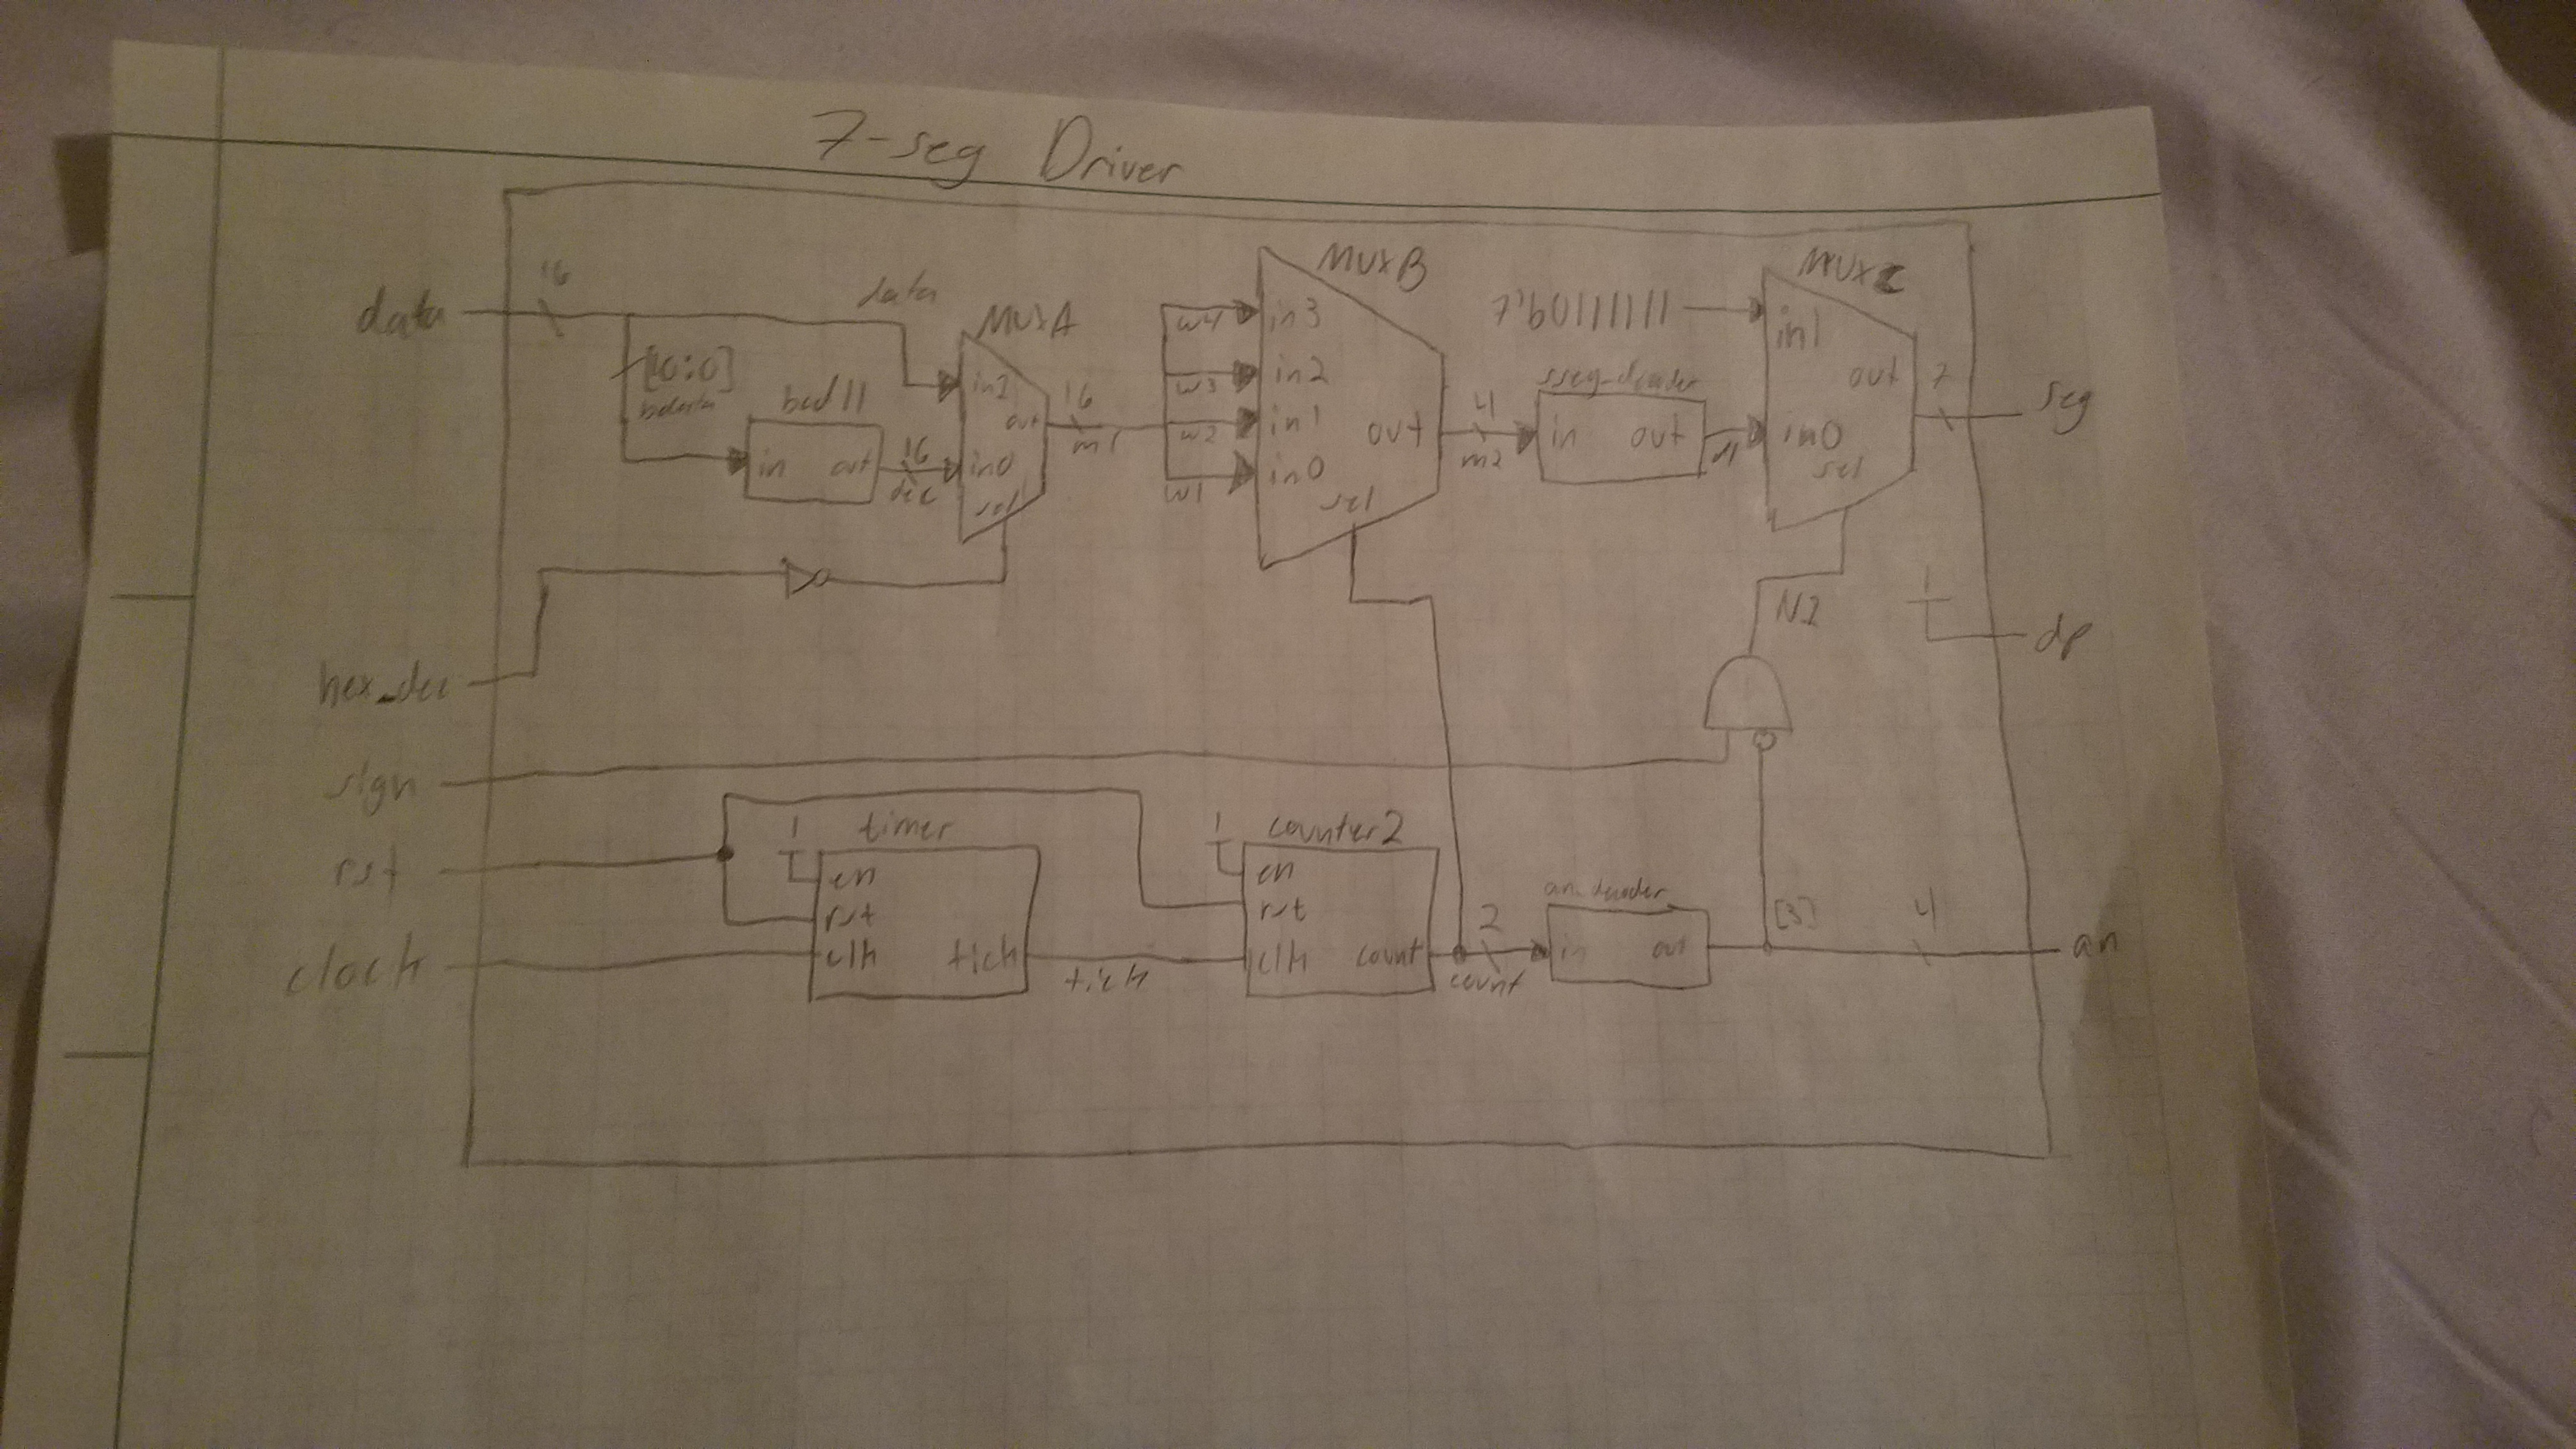
\includegraphics[width=1.0\textwidth,trim=0 0mm 0 0,clip]{7seg}
	\caption{Sseg4 TDM Schematic Drawing}
\end{figure}

\begin{figure}[ht]\centering
	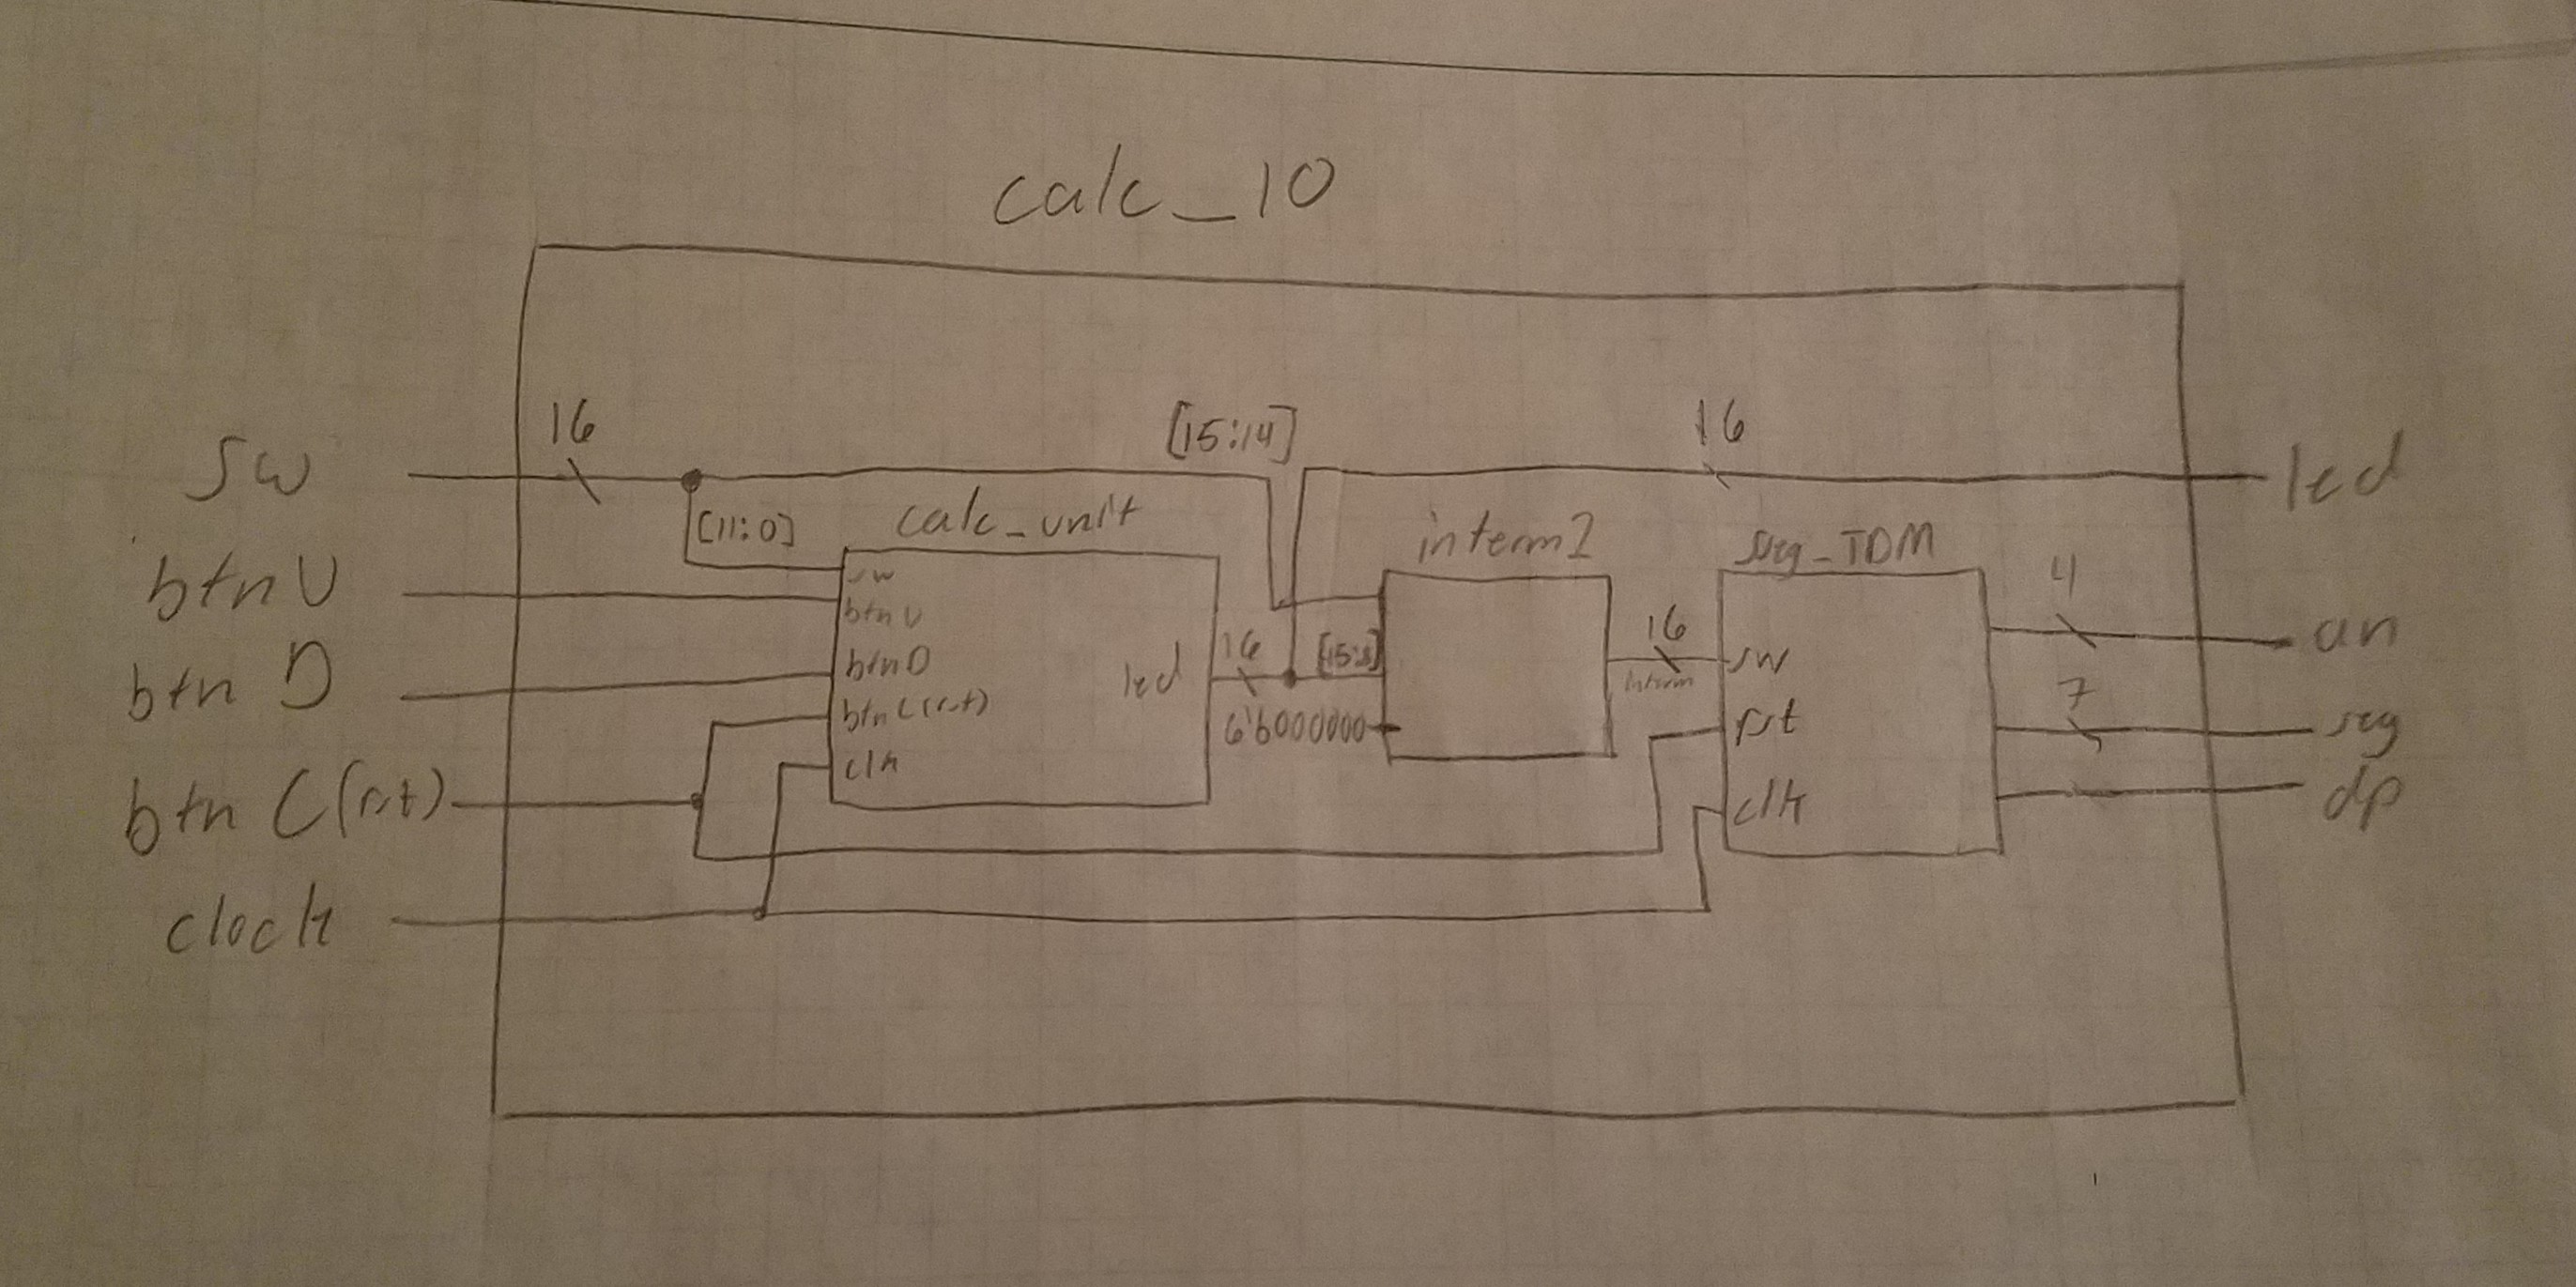
\includegraphics[width=1.0\textwidth,trim=0 0mm 0 0,clip]{calc101}
	\caption{Calc Lab10 Schematic Drawing}
\end{figure}
\clearpage

\section*{Code}

\Verilog[firstline=23,caption=Verilog Counter Source,label=code:file_ex]
{counter.sv}

\Verilog[firstline=23,caption=Verilog Sseg Source,label=code:file_ex]
{sseg4.sv}

\Verilog[firstline=23,caption=Verilog Top Lab 10 Source,label=code:file_ex]
{calc_lab10.sv}

\Verilog[firstline=23,caption=Verilog Sseg Test Bench,label=code:file_ex]
{sseg_TDM_test.sv}

\clearpage

\Verilog[firstline=23,caption=Verilog Counter Test Bench,label=code:file_ex]
{counter_test.sv}



\end{document}
